\chapter{Implementierung}
Nachdem die ersten Kontakte mit den beiden Kerntools erfolgt sind und eine geeignete Basis für das Projekt gefunden wurde, gilt es nun, dieses in die Tat umzusetzen.
Wie in \autoref{sec:einarbeitung} kann auch für das richtige Projekt eine Aufteilung der Entwicklung in Erstellung des Servers und anschließende Einbindung in das Containerimage erfolgen, was insbesondere das Testen des Servers während der Entwicklung deutlich vereinfacht und mögliche Fehlerquellen eingrenzt.

\section{Node-Server}
Angesichts dessen, dass der Node-Server im Anschluss lediglich in einen Container eingeschnürt wird, ist die Erstellung des eigentlichen Servers der deutlich größere und wichtigere Bearbeitungsschritt.
Wie bei jedem Projekt liegt auch hier der Einstiegspunkt im Errichten eines Grundgerüsts.
Im konkreten Fall bedeutet das, das node-ui5 Modul erfolgreich in Node.js zu importieren, die richtigen Konfigurationsoptionen dafür zu finden, innerhalb des Moduls den SAP Mock Server anzusteuern und diesen unkonfiguriert für externe Anfragen erreichbar zu machen.
In der Theorie klingt dies einfach.
Allerdings tritt an dieser Stelle sowohl das Problem auf, dass node-ui5 kaum dokumentiert, als auch der Mock Server nicht für solch einen Einsatz vorgesehen ist, wodurch auch die Hilfeseiten von SAP für diesen initialen Schritt nicht sonderlich hilfreich sind.

\subsection{Grundgerüst des Mock Servers}
\label{subsec:foundation}
Für das Node-Projekt wird zunächst die folgende package.json (\autoref{code:basic-ms-package.json}) angelegt.
Hier wird zunächst ein Projektname mit Versionsnummer und Kurzbeschreibung angelegt, sowie in Zeile 5 der Einstiegspunkt für die Applikation definiert.
Die drei, in Zeile 6 folgende festgelegten, Projekt-Abhängigkeiten stellen hier allerdings den primär wichtigen Teil dar.
Das \enquote{body-parser}-Paket wird dafür benötigt, um den Inhalt von Anfragen an den Server sauber verarbeiten zu können.
Mit den hauseigenen Bibliotheken von Node.js ist zwar die Erstellung von Webservern bereits möglich, dieser Prozess wird jedoch vom \enquote{Express}-Framework stark vereinfacht.
Nicht zuletzt wird noch das \enquote{node-ui5}-Modul eingebunden.
Mithilfe der hier definierten Abhängigkeiten, muss nun lediglich noch \emph{npm install} ausgeführt werden und die Implementierung des Mock Servers kann starten.
\lstinputlisting[
	label=code:basic-ms-package.json,
	caption=Package.json für das Grundgerüst (gekürzt),
	captionpos=b,
	firstline=1,
	lastline=10
]{Quellcode/basic-ms/package.json}

Nachfolgend wir in \autoref{code:basic-ms-mockserver.js} der Quellcode der mockserver.js dargestellt.
Beginnend muss node-ui5 eingebunden werden (Zeile 1).
Dies geschieht hier unter Verwendung der mitgelieferten \enquote{factory}, die einige Konfigurationsschritte beim Einbinden direkt übernimmt.
Parameter, die sie dabei berücksichtigen soll, werden in den folgenden 3 Zeilen gesetzt, unter anderem die Variable myApp, als Referenz auf das Verzeichnis, in dem die mockserver.js liegt.
Nachdem node-ui5 in Node eingebunden wurde, wird nun der gesamte folgende Code als Callback-Funktion der Einbindung ausgeführt.
So enthält Zeile 7 bereits SAPUI-Code, welcher weitere SAPUI-Module einbindet (hier MockServer), welche in Zeile 9 einer anschließend automatisch ausgeführten Funktion übergeben werden.

\paragraph{Konfiguration des Mock Servers}
Ab Zeile 10 wird der eigentliche Mock Server initialisiert.
Hierzu wird zunächst in der Variable \emph{ms} ein neues Mock Server Objekt erstellt, welches für den gesamten Subpfad von \enquote{/} zuständig ist.
Zeile 14 folgende teilen dem Mock Server mit, wo er die Daten findet, die er simulieren soll (myApp/mockdata), wie diese strukturiert sind (myApp/metadata.xml) und ob automatisch Platzhalter für fehlende Daten generiert werden sollen.
Zeile 19 bis 21 nehmen schließlich noch die Einstellung vor, dass der Mock Server automatisch antwortet und in diese Antwort eine künstliche Verzögerung einbaut, um die Simulation realistischer zu gestalten, bevor der Mock Server in Zeile 24 gestartet wird.

\paragraph{Externe Freigabe}
Nun läuft der Mock Server zwar und wurde mit Datensätzen versorgt, die er simulieren kann, jedoch ist er noch nicht für Anfragen außerhalb der Node.js-Umgebung erreichbar.
Zu diesem Zweck wird nun ab Zeile 26 noch ein zusätzlicher Webserver mithilfe des Express-Framework eingerichtet.
Zunächst werden hierzu die mit \ac{npm} installierten Module geladen und eine neue Express-Applikation initialisiert.
Das zusätzlich installierte Modul für den body-parser wird nun als Standardparser für Anfragen an den Express-Server konfiguriert (Zeile 30 folgende).
Anschließend wird eine Funktion festgelegt, die für jede Anfrage eines beliebigen Typs (GET, POST, PUT, ...) ausgeführt wird, die an den Express-Server geschickt werden (Zeile 35) und zwar sollen diese alle an den Mock Server weitergeleitet werden.
Der Mock Server ist so implementiert, dass er automatisch alle \ac{AJAX}-Anfragen abfängt.
Somit kann direkt basierend auf den Daten und Parametern der ursprünglichen Anfrage eine solche erstellt werden (Zeile 36-40).
Der \ac{AJAX}-Anfrage wird eine Callback-Funktion übergeben, die ausgeführt wird, wenn die Antwort des Mock Servers auf die Anfrage erfolgt ist.
In dieser werden zunächst sämtliche Header-Daten aus der \ac{AJAX}-Antwort in die Antwort des Express-Servers auf die externe Anfrage kopiert.
Letztere wird anschließend noch mit dem Status-Code der \ac{AJAX}-Response versehen und mit deren Text zurück an den externen Client geschickt (Zeile 41-51).
Übrig bleibt nur noch das Starten des Express-Servers (Zeile 56).
\lstinputlisting[
	label=code:basic-ms-mockserver.js,
	caption=Quellcode des Grundgerüsts (mockserver.js),
	captionpos=b
]{Quellcode/basic-ms/mockserver.js}

\subsection{Function Imports}
Zum aktuellen Zeitpunkt ist es bereits gelungen, einen lauffähigen OData-Service zu errichten, welcher externe Anfragen beantwortet.
Damit dieser nun als neuer \ac{ewm-sim} dienen kann, muss er allerdings zunächst mit den richtigen Mockdaten versorgt werden.
Zu diesem Zweck muss dem Server über die \emph{metadata.xml} mitgeteilt werden, wie die Datenstrukturen und Zusammenhänge zwischen diesen aussehen, die er darstellen soll.
Da der \ac{ewm-sim} eine genaue Nachbildung eines vollständigen \ac{EWM}-Systems sein soll, sind auch die Metadaten mit einem solchen übereinstimmend.
Infolge dessen kann die \emph{metadata.xml} ohne Veränderungen direkt von einem bestehenden \ac{EWM}-System übernommen werden.
Auch die darzustellenden Mockdaten haben noch dieselbe Struktur wie beim \ac{ewm-sim} in der ersten Version.
Um Mock- und Metadaten zu verändern, müssen die jeweiligen Dateien lediglich in die entsprechenden Verzeichnisse gelegt werden, welche in \autoref{subsec:foundation} konfiguriert wurden.
\todo{Code von Meta- und Mockdaten einfügen?}

In den Metadaten werden für den vollständigen Funktionsumfang des Mock Servers jedoch überdies noch Function Imports definiert.
Diese Funktionen stellen Anfragen dar, welche erweiterte Operationen beim Server auslösen, als ausschließlich einen Datensatz zu liefern oder zu manipulieren.
Für die normalen Mockdaten benötigt der Server nicht mehr als die Daten und den entsprechenden Eintrag in den Metadaten.
Bei Function Imports funktioniert das nicht so einfach, hier ist in den Metadaten lediglich festgelegt, dass eine solche Funktion zu existieren hat, auf welche \ac{HTTP}-Methode diese zu reagieren hat, welche Parameter sie entgegennimmt und was sie für einen Wertetyp zurückliefert.
Die eigentliche Funktionalität muss jedoch für jede Funktion einzeln von Hand implementiert werden.
Wie solch eine Implementierung aussieht, soll hier am Beispiel der Funktion \emph{SetRobotStatus} gezeigt werden.

\lstinputlisting[
	language=xml,
	label=code:metadata-setrobotstatus,
	caption=Metadaten der Funktion SerRobotStatus,
	captionpos=b
]{Quellcode/setrobotstatus.xml}

In \autoref{code:metadata-setrobotstatus} ist der für die Methode relevante Ausschnitt aus der \emph{metadata.xml} zu sehen.
Diesem kann entnommen werden, dass sich die Operation der Methode auf das \enquote{RobotSet} bezieht und die Methode auf \ac{HTTP}-POST-Anfragen reagieren soll.
Die Methode erwartet drei Parameter (Lgnum, Rsrc, Exccode) vom Typ String mit einer jeweils festgelegten, maximalen Länge.

Um jedoch den genauen Ablauf der Methode im Mock Server implementieren zu können, muss die Implementierung aus dem ABAP-Backend eines richtigen \ac{EWM}-Systems analysiert und in Node.js portiert werden.
Dies ist überdies wichtig, da die importierten Funktionen bestimmte Fehlercodes zurückliefern, die für den Betrieb der Roboter ebenfalls essenziell sind.

\begin{figure}[ht]
	\centering
	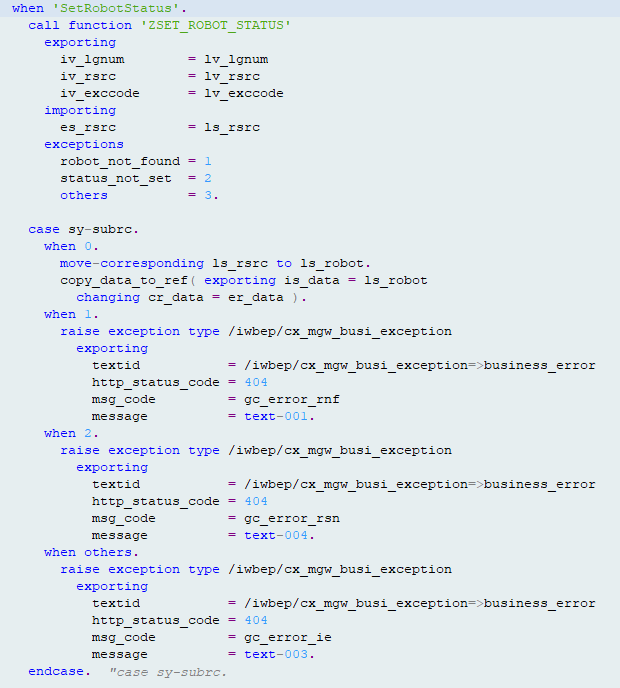
\includegraphics[width=\textwidth]{Bilder/ABAP/2020-12-04 10_20_43-Class Builder Class ZCL_ZEWM_ROBCO_DPC_EXT Display_cut.png}
	\caption{SetRobotStatus im SAP Gateway Service Builder}
	\label{fig:gwse}
\end{figure}

\autoref{fig:gwse} zeigt einen Ausschnitt aus dem \emph{SAP Gateway Service Builder}.
(Vollständige Screenshots werden aus Gründen der Lesbarkeit nicht dargestellt.)
Empfängt der OData-Service den Aufruf von \emph{SetRobotStatus}, ruft er intern im Backend die Methode \emph{ZSET\_ROBOT\_STATUS} mit den mitgegebenen Parametern auf.
Die Methode kann zwei klar definierte und eine sonstige Exception zurückliefern.
Diese Exceptions werden Exitcodes zugeordnet und anschließend wird eine Fallentscheidung anhand dieser Rückgabewerte durchgeführt.
Kommt es beispielsweise zur \emph{robot\_not\_found}-Exception, so wird vom OData-Service eine Antwort mit dem \ac{HTTP}-Statuscode \emph{404} zurückgegeben.
Der Nachrichteninhalt wird durch die Konstante \emph{gc\_error\_rnf} festgelegt.
Um von dieser den eigentlichen Wert abzurufen, muss im Class Builder (\autoref{fig:class-builder}) nachgeschlagen werden.
Dort steht zu jeder Konstante (Attribute) der zugehörige Wert des Fehlercodes (Initial Value).

\begin{figure}[ht]
	\centering
	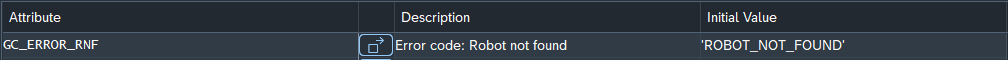
\includegraphics[width=\textwidth]{Bilder/ABAP/2020-12-04 10_22_23-Class Builder_ Display Class ZCL_ZEWM_ROBCO_DPC_EXT_cut.png}
	\caption{Fehlercodes im Class Builder}
	\label{fig:class-builder}
\end{figure}


\subsection{Authentifizierung}

\subsection{Unit-Tests}


\section{Erstellung des Dockerimages}


\section{Automatisierte Tests mit Travis-CI}


\section{Deployment in \ac{GKE}}